\newpage
\section{Microservices}

Microservice is an approach to Distributed Systems to build an application
as a set of smaller autonomous services. In this architecture, services (SOA\footnote{SOA: Service Oriented Architecture}) \cite[chapter ~3]{SOA}
are lightweight and Domain Driven \cite{DDD} that makes the application simple to understand, develop and test. The smaller set of services
can be developed autonomously by different teams and be deployed independently. This brings loose coupling within a system, 
since the application is decentralized.

Figure \ref{fig:monolithVsMicro} shows the core difference for deployment between a Monolithic and a Microservice architecture. 
It is clear that from the figure, in a Monolithic application, if a small change is made, the whole application has to be deployed again completely as 
opposed to the Microservice architecture. The Microservice approach allows a rapid development, since only the desired services
can be changed and deployed independently. This way the developing teams also have an hand on advantage to carry out different
continuous integration practices in isolation.


\begin{figure}[htbp!]
    \centering 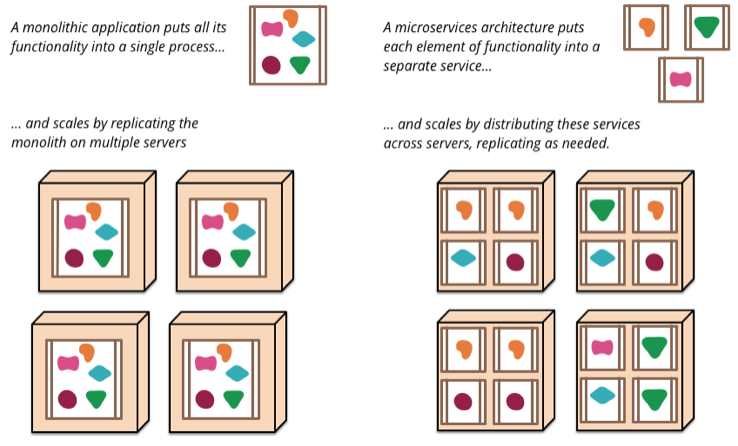
\includegraphics[scale=0.6]{grafiken/monolithVsMicro.png}
    \caption{ Monolithic vs Microservice deployment approach \cite{FowlerMartin}}
    \label{fig:monolithVsMicro}
\end{figure}

\newpage
Figure \ref{fig:serviceExample} shows an example of how 
a service is domain bounded and there is a flexibility of choosing different
technologies for the isolated services \cite{MicroserviceNewMan}. 
Each service is encapsulated with their own life cycles, which communicates with each other using protocols 
(e.g. HTTP \cite{HTTP}, websockets \cite{WebSockets}, GRPC \cite{grpc}). 

\begin{figure}[htbp!]
    \centering 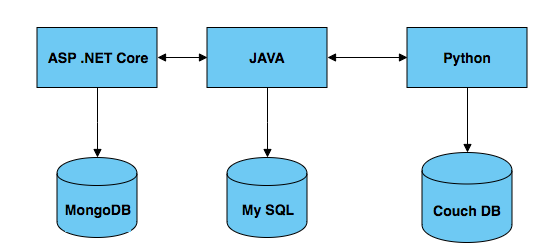
\includegraphics[scale=0.3]{grafiken/microservices.png}
    \caption{ Illustration of services as independent entities \cite{MicroserviceNewMan}}
    \label{fig:serviceExample}
\end{figure}

\par
    Comparing microservices to a single monolithic application \cite[p.~94]{{softwareDesign}} where the
    system is built as a large single unit and runs in a single process. 
    This is considered the most natural way to develop a server side 
    application. It is seen that as the application scales in size, it 
    gets harder to keep up with the changes. As scaling requires the whole
    application to be scaled as a whole. This is where microservices come very handy,
    as the only the required bounded module can be scaled up as needed. 
    There are factors to be considered before going for a microservice
    architecture.

    \begin{table}[h!]
        \centering
        \begin{tabular}{|p{9cm}|p{7.5cm}|}
            \hline
                \textbf{Advantages}  & \textbf{Disadvantages}\\
            \hline
                The services can be developed with different languages & 
                A mature team must be present to maintain large number of services \\
            \hline
                A strong modular boundaries is present which reinforces a modular
                structure.
                & All the services must manage eventual consistency which is
                harder to manage in a large distributed system.\\
            \hline
                 Independent deployment is easier since the services are
                 autonomous. & Harder to program since remote calls must be made.\\
            \hline
        \end{tabular}
        \caption{Advantages and disadvantages of microservices \cite{FowlerMartin}}
        \label{table:Advantages and disadvantages of microservices}     
    \end{table}    

    \newpage
    \subsection{Data Sovereignty In Microservice}
    \label{subsection:dataSovereignty}
    It is an important guideline for a Microservice architecture to own its domain data and 
    logic \cite[p.~29]{Torre2017}. Decentralized Data would assist a single Microservice
    to become solely independent and help them evolved individually. The approach of each Microservice owning its own database is also
    know as \textbf{Polyglot Persistence} \cite{Polyglot}. Applying this pattern would imply that the
    data belonging to one service is available to the others only via the API of the Microservice.

    \begin{figure}[H]
        \centering 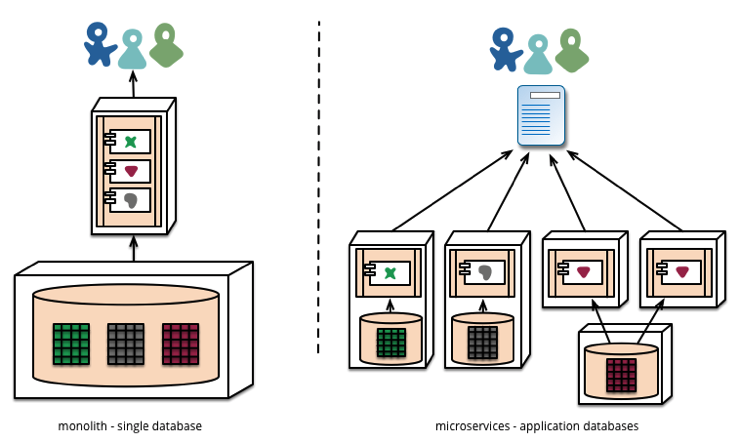
\includegraphics[scale=0.5]{grafiken/polyglot.png}
        \caption{Data management approach in a Monolithic application vs Microservice \cite{FowlerMartin}}
        \label{fig:polyglot}
    \end{figure}
    
   In Figure \ref{fig:polyglot}, it can be observed how a Monolithic application owns only a single database for the whole application. Meaning,
   the application is sharing all data across multiple domains and has tight coupling with each other. Whereas, in Microservices each service owns
   a single database which is easier to manage. Having said that data sovereignty is very beneficial, it also brings various difficulties
   i.e. coordinations between services, which are very challenging to tackle and creates data coherency issues in the system. 




